\section{Экономический раздел}
\label{sec:economy}

\subsection{Описание ниши и специфики программного продукта}

Программный комплекс организации и выдачи верифицированных цифровых дипломов на базе блокчейна ориентирован на выпуск и управления цифровых дипломов в формате невзаимозаменяемых (NFT, Non-Fungible Tokens) и «привязанных к душе» (SBT, Soulbound Tokens) токенов.

ПК ориентирован на образовательные учреждения, академические институты, сертификационные центры, консалтиноговые и коммерческие организации, предлагая средство для выпуска дипломов, сертификатов и других документов в цифровом виде с использованием технологии блокчейн, что позволяет обеспечить высокий уровень защиты данных и исключить возможность фальсификации документов.

Требуемый объем и состав программных средств для управления цифровыми дипломами и сертификатами через блокчейн включает серверное приложение для подготовки и формирования данных, смарт-контракт в децентрализованной сети блокчейна, клиентские приложения для запроса и просмотра дипломов.

Продукт относится к классам прикладного программного обеспечения (05.10) и отраслевого прикладного программного обеспечения (12.15, 12.17)~\cite{bib:reestrpo}. Решение совместимо с ЭВМ на базе процессоров с архитектурой AMD, ARM (32/64 bit) и операционными системами Windows 7, OS X 10.9 Mavericks, Linux 3.16 (в том числе Astra и Alt), Android 9 и новее.

Сложность разработки продукта --- средняя, включает разработку собственных решений и интеграцию типовых модулей. Возможно применение стандартных и проверенных технологий для обеспечения стабильности работы и безопасности данных. Предполагаемое время разработки --- 720 часов, а стоимость порядка 3.000.000 рублей, включая расходы на разработку, тестирование, доработку и поддержку ПП.

\subsection{Оценка трудозатрат по разработке ПО согласно модели COCOMO II}

В рамках оценки затрат на разработку и внедрение программного обеспечения применялась модель COCOMO II~\cite{bib:cocomoii_gen, bib:cocomoii_win}, представляющая собой алгоритм для определения стоимости создания ПО. Эта модель предлагает ряд преимуществ и предоставляет детализированное описание методик настройки и проведения оценок. COCOMO II использует упрощенную регрессионную формулу, основанную на данных из различных проектов, и поддерживает разнообразие жизненных циклов проектов и языков программирования. Оценка трудозатрат и времени, необходимого для разработки, помогает планировать бюджет, определять оптимальные сроки и стоимость реализации программного продукта.

Процесс оценки в COCOMO II разделяется на два этапа: предварительная оценка в начале проекта и более детальная оценка после разработки архитектуры. В экономическом разделе выпускной квалификационной работы учитывается только предварительная оценка по модели COCOMO II.

Формула~\ref{eq:pm}, предназначенная для оценивания трудозатрат ($PM$), имеет следующий вид:
\begin{equation}
    PM = EAF \times A \times SIZE^E,
    \label{eq:pm}
\end{equation}

где $EAF$ (Effort Adjustment Factor) --- произведение выбранных множителей трудоемкости по всем критериям из формулы~\ref{eq:eaf};

$A$ --- корректирующий коэффициент, который на этапе предварительной оценки считается равным 2,94;

$SIZE$ --- объем программного продукта в тысячах строк исходного текста (KSLOC --- Kilo of Source Line of Code);

$E$ --- фактора масштаба, влияющего на нелинейность в зависимости трудоемкости проекта от его размераб формула~\ref{eq:e};
\begin{equation}
    EAF = \prod_{i=1}^n EM_i,
    \label{eq:eaf}
\end{equation}

где $EM_i$ (Effort Multiplier) --- коэффициент множителя трудоемкости;

$n$ --- количество критериев оценки (для предварительной оценки количество факторов в модели равно 8);
\begin{equation}
    E = B + 0.01 \times \sum_{j=1}^5 SF_j,
    \label{eq:e}
\end{equation}

где $B$ --- корректирующий коэффициент, который на этапе предварительной оценки принимается за 0,91;

$SF_j$ (Scale Factors) --- коэффициенты масштабирования.

\subsubsection{Оценка готовности к коммерциализации}

В рамках анализа готовности к коммерциализации программного продукта, проведена оценка ключевых параметров, определяющих его готовность к выходу на рынок. Этот процесс включает в себя анализ различных аспектов, как соответствие требованиям и ожиданиям целевой аудитории, качество и удобство интерфейса, функционирование, уровень документации и безопасности, а также перспективы бренда и качество обслуживания. Выделение данных критериев позволяет не только выявить текущее состояние продукта, но и определить необходимые шаги для его оптимизации и улучшения с точки зрения потребителей и рыночных требований.

\begin{table}[H]
    \caption{Оценка готовности к коммерциализации}
    \centering

    \tolerance=0
    \emergencystretch=10pt
    \hyphenpenalty=0
    \exhyphenpenalty=0
    \begin{tabular}{@{}ll@{}}
        \toprule
        \textbf{Наименование критерия}                    & \textbf{Оценка} \\ \midrule
        Соответствие ожиданиям целевой группы & 5 \\
        Качество интерфейса & 3 \\
        Работоспособность и стабильность & 5 \\
        Полнота документации & 2 \\
        Комплексная безопасность & 4 \\
        Ожидаемый эффект от внедрения & 5 \\
        Известность бренда производителя & 3 \\
        Качество сервиса и обслуживания & 5 \\ \midrule
        Коэффициент степени готовности к коммерциализации & 0,8 \\ \bottomrule
    \end{tabular}
    \label{tab:prepare_mark}
\end{table}

Аргументация оценки готовности к коммерциализации:
\begin{enumerate}
    \item Соответствие ожиданиям целевой группы --- 5, поскольку продукт удовлетворяет требованиям и пожеланиям целевой группы.
    \item Качество интерфейса --- 3, из-за того, что для администратора системы предназначен только интерфейс командной строки (CLI), а для пользователя разработан минималистичный интерфейс в виде кнопок и текстовых команд, интегрированный в Telegram.
    \item Работоспособность и стабильность --- 5, поскольку система взаимодействует с децентрализованными сервисами и может использовать многочисленные точки входа, в случае отказа стандартных.
    \item Полнота документации --- 3, в связи с тем, что присутствует только необходимая для регистрации продукта в реестре российского ПО документация~\cite{bib:reestrpo_docs}.
    \item Комплексная безопасность --- 4, персональные данные пользователей не хранятся и не публикуются в явном виде, но абсолютной безопасности не существует;
    \item Ожидаемый эффект от внедрения --- 5, потому что целевая аудитория заинтересована проектом во время проведения опроса на ранней стадии разработки и проектирования;
    \item Известность бренда производителя --- 3, поскольку это дебютный проект организации в данной сфере.
    \item Качество сервиса и обслуживания --- 5, продукт полностью автоматизирован и имеет замкнутый цикл работы.
\end{enumerate}

Таким образом, исходя из оценок в таблице~\ref{tab:prepare_mark}, программный продукт демонстрирует высокий уровень готовности к коммерциализации в виде коэффициента готовности, рассчитанного по формуле~\ref{eq:eaf}, в размере 0.8, что соответствует готовности к выходу на рынок.

$$EAF = \frac{\left(\frac{5 + 3 + 5 + 2 + 4 + 5 + 3 + 5}{8}\right) \times 2}{10} = 0.8$$

Продукт уже обладает сформированным спросом и конкурентными преимуществами, что способствует его успешной реализации в существующих рыночных условиях. Однако, для успешной коммерциализации, следует уделить внимание полноте технической документации, известности бренда и четкому позиционированию на рынке, акцентируя внимание на уникальных характеристиках и преимуществах перед аналогами. Это позволит максимизировать рыночный потенциал и обеспечить устойчивое развитие.

\subsubsection{Оценка фактора масштаба}

Модель оценки фактора масштаба состоит из следующих ключевых элементов:

\begin{enumerate}
    \item PREC --- прецедентность, наличие схожего опыта;
    \item FLEX --- гибкость процесса разработки;
    \item RESL --- архитектура и разрешение рисков;
    \item TEAM --- сработанность команды;
    \item PMAT --- зрелость процессов.
\end{enumerate}

Эта оценка важна для анализа и понимания того, как различные переменные влияют на общий результат или процесс.

\begin{table}[H]
    \caption{Оценка трудозатрат по разработке ПО согласно модели COCOMO II}
    \centering

    \tolerance=0
    \emergencystretch=10pt
    \hyphenpenalty=0
    \exhyphenpenalty=0
    \begin{tabular}{@{}ll@{}}
        \toprule
        \textbf{Оценка фактора масштаба (j)} & \textbf{Значение} \\
        PREC & 3.72 \\
        FLEX & 1.01 \\
        RESL & 1.41 \\
        TEAM & 1.10 \\
        PMAT & 3.12 \\
        \midrule
        SF$_j$ & 10.36 \\
        E & 1.0136 \\
        \bottomrule
    \end{tabular}
    \label{tab:scale_factor}
\end{table}

Уровни значимости~\cite[c. 22-24]{bib:scale_f}, обозначаемые как ($SF_j$), были опытным путем оценены и занесены в таблицу~\ref{tab:scale_factor}.

\begin{enumerate}
    \item PREC --- средний, есть опыт в применяемых технологиях и опыт разработки продуктов для рассматриваемой сферы;
    \item FLEX --- очень высокий, но имеется незначительная жесткость;
    \item RESL --- очень низкий, 90\% рисков известны и заложены;
    \item TEAM --- очень высокий, сработанность команды на хорошем уровне;
    \item PMAT --- высокий, модель зрелости возможностей на хорошем уровне (CMM Уровень 3).
\end{enumerate}

Основываясь на данных из таблицы~\ref{tab:scale_factor}, по формуле~\ref{eq:e} получаем значение фактора масштаба равное 1.0136.
$$E = 0.91 + 0.01 \times (3.72 + 1.01 + 1.41 + 1.1 + 3.12) = 1.0136$$

\subsubsection{Оценка фактора трудоемкости}

Модель оценки фактора трудоёмкости ($EMj$) состоит из перечисленных далее элементов~\cite{bib:labor_f}:

\begin{enumerate}
    \item PERS --- квалификация персонала;
    \item PREX --- опыт персонала;
    \item RCPX --- сложность и надежность продукта;
    \item RUSE --- разработка для повторного использования;
    \item PDIF --- сложность платформы разработки;
    \item FCIL --- оборудование (инструменты простейшие/интегрированные средства поддержки жизненного цикла);
    \item CSED --- требуемое выполнение графика работ;
    \item SIZE --- объем программного продукта в тысячах строк исходного текста (KSLOC).
\end{enumerate}

Объем продукта рассчитывается с использованием метода PERT или за счет анализа продукта на основе функциональных точек. В рамках выпускной квалификационной работы для расчета объема продукта можно воспользоваться данными из таблицы~\ref{tab:labor_factor}.

\begin{table}[H]
    \caption{Оценка фактора трудоемкости согласно модели COCOMO II}
    \centering

    \tolerance=0
    \emergencystretch=10pt
    \hyphenpenalty=0
    \exhyphenpenalty=0
    \begin{tabular}{@{}ll@{}}
        \toprule
        \textbf{Оценка фактора трудоемкости ($EMj$)} & \textbf{Значение} \\
        \midrule
        PERS & 1.00 \\
        PREX & 1.00 \\
        RCPX & 1.00 \\
        RUSE & 1.24 \\
        PDIF & 1.00 \\
        FCIL & 1.30 \\
        CSED & 1.14 \\
        SIZE & 2.00 \\
        \midrule
        EAF & 1.83768 \\
        PM & 10.91 \\
        \bottomrule
    \end{tabular}
    \label{tab:labor_factor}
\end{table}

Оценка факторов трудоемкости ($EMj$) программного продукта опытным путем показала следующие значения функциональных точек:

\begin{enumerate}
    \item PERS --- нормальный, персонал достаточно квалифицирован для выполнения поставленных задач;
    \item PREX --- нормальный, имеется опыт в реализации подобных продуктов;
    \item RCPX --- нормальный;
    \item RUSE --- супер высокий, решение можно будет использовать повторно;
    \item PDIF --- нормальный;
    \item FCIL --- очень низкий, оборудование необходимо закупить;
    \item CSED --- низкий.
\end{enumerate}

Исходя из приведенных в таблице~\ref{tab:scale_factor} данных, по формулам~\ref{eq:eaf} и~\ref{eq:pm} получаем следующие значения:
$$EAF = 1 \times 1 \times 1 \times 1.24 \times 1 \times 1.3 \times 1.14 = 1.83768$$
$$PM = 1.83768 \times 2.94  \times 2^{1.0136} = 10.91 \text{ мес./чел.}$$

Таким образом, полученное значение 10.91 мес./чел. говорит о том, что данный проект может быть выполнен за 11 целых месяцев --- одним человеком или за полгода группой из двух человек ($10.91/2=5.455$).

\subsection{Оценка стоимости разработки программного продукта}

Оценка стоимости разработки программного продукта производится согласно формуле~\ref{eq:pp_cost}:
\begin{equation}
    P_r = PM \times W,
    \label{eq:pp_cost}
\end{equation}

где $P_r$ обозначает стоимость разработки ПО, $W$ --- средняя заработная плата участвующих в разработке сотрудников, а $PM$ --- трудозатраты, выраженные в количестве месяцев.

Используя ранее полученные значения, расчитаем стоимость разработки по вышеуказанной формуле:
$$P_r = 10.91 \times 120000 = 1309200$$

\subsection{Расчет полной стоимости программного продукта (в части трудозатрат)}

При оценке общей стоимости создания программного продукта необходимо учитывать не только трудозатраты программистов, но и затраты на других специалистов. Это включает анализ требований, проектирование функциональных возможностей, архитектуры и пользовательских интерфейсов, создание документации и плана интеграции, а также проведение тестирования. В процессе разработки программного обеспечения задействованы не только разработчики, но и тестировщики, технический писатель и другие ключевые участники. Обычно на каждый час работы разработчиков приходится около одного часа труда других специалистов, участвующих в подготовке и поддержке проекта.

Среднее временных затрат специалистов~\cite{bib:cost_dis}:

\begin{enumerate}
    \item Проектирование занимает 35\% относительно времени разработки.
    \item Тестирование занимает около 55\%.
    \item На техническое сопровождение и внедрение уходят 10\%.
\end{enumerate}

\begin{table}[H]
    \caption{Расчёт полной стоимости программного продукта в части трудозатрат}
    \centering

    \tolerance=0
    \emergencystretch=10pt
    \hyphenpenalty=0
    \exhyphenpenalty=0
	\begin{tabular}{x{3cm}x{2.75cm}x{2.75cm}x{2.75cm}x{2.75cm}}
		\toprule
		\textbf{Сотрудники (i)} & \textbf{Процент затрат времени на работу i-го специалиста, \%} & \textbf{Трудозатраты, количество мес. PM} & \textbf{Средний оклад, руб.} & \textbf{Приведенные затраты специалистов, руб.} \\ \midrule
		Проектирование (Проектировщик) & 35 & 3.82 & 90000 & 343598.91 \\
		Разработка (Разработчик) & 100 & 10.91 & 120000 & 1308948.23 \\
		Тестирование (Тестировщики) & 50  & 5.45 & 60000 & 327237.06 \\
		Нагрузочное тестирование (Внедрение) & 5 & 0.55 & 120000 & 65447.41 \\
		Внедрение (Внедрение) & 5 & 0.55 & 120000 & 65447.41 \\
		Техническая документация (Производство) & 5 & 0.55 & 60000 & 32723.71 \\
        \midrule
		\multicolumn{4}{l}{Итого полная стоимость ПО в части трудозатрат} & 2143402.72 \\ 
		\bottomrule
	\end{tabular}
	
	\label{tab:cost_work_time}
\end{table}

Получается, что полная стоимость программного продукта (в части трудозатрат), с полным циклом и количеством специалистов равным 6 ($i=6$), составила 2 млн. 143 тыс. 400 рублей.

\subsection{Оценка стоимости разработки и внедрения программного продукта}

Согласно методологии, оценка стоимости трудозатрат на программное обеспечение включает в себя общую сумму заработной платы с добавлением 13\% налога на доходы. Также, помимо базовой заработной платы, необходимо учесть и дополнительные расходы, которые могут быть как обязательными, так и опциональными.

Например:

\begin{enumerate}
    \item Выплаты премий до 15\% от зарплаты;
    \item Обязательные страховые в размере 7,6\%;
    \item Возмещение расходов на питание до 2\%.
\end{enumerate}

Кроме того, работодатель обязан обеспечить сотрудникам должные условия труда, включая офисное оборудование и средства коммуникации. Из-за этого формируются дополнительные расходы, приведенные в таблице~\ref{tab:calculation_expenses_software_development}.

\begin{table}[H]
	\caption{Оценка стоимости разработки и внедрения программного продукта}
	\centering
	
	\tolerance=0
	\emergencystretch=10pt
	\hyphenpenalty=0
	\exhyphenpenalty=0
	\begin{tabular}{x{7cm}x{3cm}x{3cm}}
		\toprule
		\textbf{Статьи калькуляции} & \textbf{Процент расходов} & \textbf{Сумма} \\ \midrule
		Полная стоимость ПО в части трудозатрат & {-} & 2143402.72 \\
		Расходы на хозяйственные и административные нужды & 20\%   & 428680.544 \\
		Премия к заработной плате & 15\%   & 321510.408 \\
		Компенсация питания сотрудников & 2\%    & 42868.0544 \\
		Взносы на социальное страхование & 7.60\% & 223171.0912 \\
		\multicolumn{2}{l}{Полная стоимость внедрения ПО, в т.ч. НДС 0\%} & 3159632.818 \\ \bottomrule
	\end{tabular}
	
	\label{tab:calculation_expenses_software_development}
\end{table}

При расчете финальной стоимости внедрения также требуется учесть налог на добавленную стоимость (НДС) в размере 20\% от общей суммы, но, учитывая, что программный продукт будет внесен в реестр отечественного ПО, то НДС равен 0\%. Таким образом, полная стоимость разработки и внедрения ПП составит 3 млн. 159 тыс. 633 рубля.

\subsection{Расчет общего количества капитальных затрат ТСО (CAPEX)}

Согласно методологии общей стоимости владения (TCO) от Gartner~\cite{bib:tco_gartner}, при оценке капитальных затрат учитываются не только инвестиции на внедрение программного продукта, но и затраты на техническую поддержку и консультации, необходимые для адаптации системы под потребности компании. Важно также принимать во внимание расходы на обучение сотрудников и приобретение специализированного оборудования и информационного канала для стабильной работы корпоративной ИС.

Часто организации не включают эти статьи расходов в проектный бюджет, что ведет к недооценке общей стоимости продукта. Такие затраты следует учитывать при подсчете окончательной суммы капитальных вложений.

Расчет затрат на обучение и повышение квалификации персонала может быть выполнен на основе данных анализа многочисленных проектов по разработке и внедрению программного обеспечения в различных, включая иностранные, компаниях. Исследования показывают, что расходы на обучение обычно не превышают 20\% от общей стоимости внедрения программного решения.

Таким образом, зная начальные капитальные затраты (полная стоимость внедрения ПО) и установленный предел в 20\%, можно вычислить максимально возможную сумму, которую компания может включить в общую стоимость владения как расходы на обучение и подготовку персонала.
$$K_{\text{пк.}} = 3159632.82 \times 20\% = 631926.57 \text{ руб.}$$

Согласно этому пропорциональному методу, предполагаемые затраты на обучение персонала оцениваются в 632 тысячи рублей.

\subsection{Калькуляция затрат на закупку специального оборудования или каналов связи}

\subsection{Расчет общего количества операционных затрат ТСО (OPEX)}

\subsection{Расчет совокупной стоимости владения (ТСО)}

\subsection{Оценка конкурентоспособности программного продукта}

\begin{figure}[H]
	\centering
	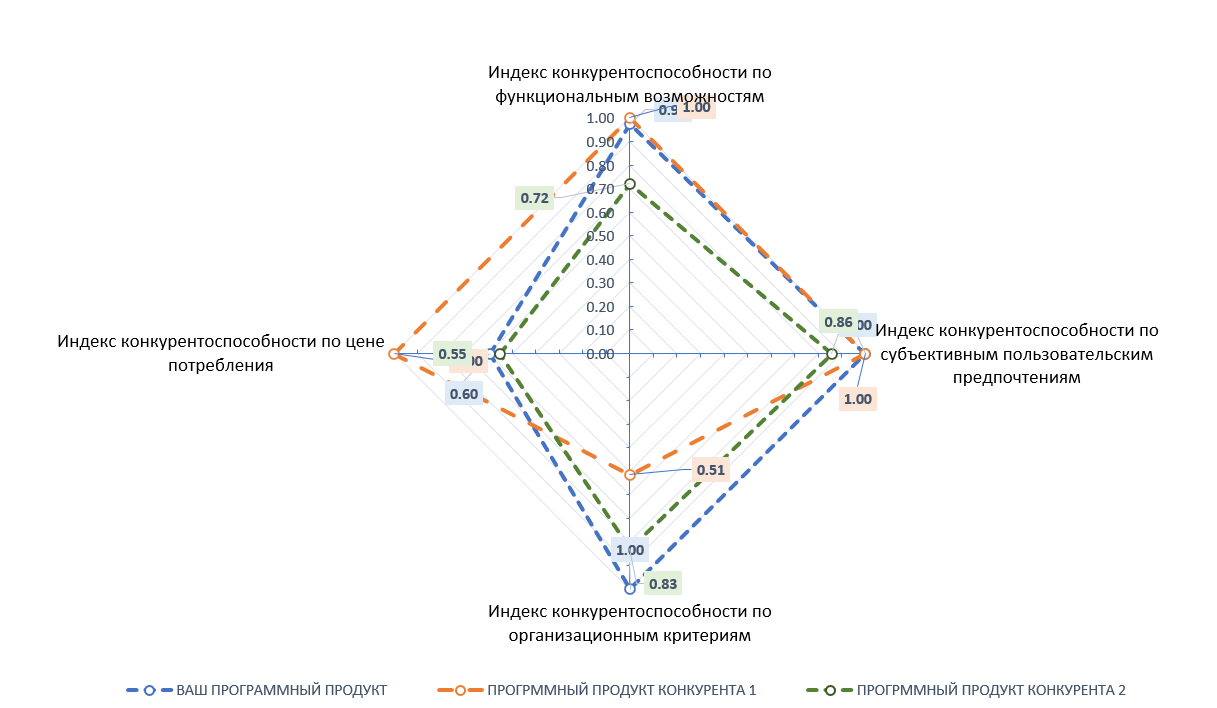
\includegraphics[width=\textwidth]{images/ec_competitive_chart.png}
	\parskip=6pt
	\caption{Диаграмма направленности конкурентоспособности ПП}
	\label{fig:competitive}
\end{figure}